%
% software.tex
%
% Copyright (C) 2015, Achim Lösch <achim.loesch@upb.de>, Christoph Knorr <cknorr@mail.uni-paderborn.de>
% All rights reserved.
%
% This documentation may be modified and distributed under the terms
% of the BSD license. See the LICENSE file for details.
%
% encoding: UTF-8
% tab size: 4
%
% author: Achim Lösch (achim.loesch@upb.de)
% created: 7/24/14
% version: 0.5.8 - change project name to ampehre
%          0.6.0 - add ioctl for the ipmi timeout, new parameters to skip certain measurements 
%                  and to select between the full or light library. 
%

\section{Software Framework}\label{sec:SoftwareArchitecture}

In this section we first describe how to build and install our measuring framework. Secondly, we give a brief overview of libmeasure's modular software architecture. Finally, we explain what you have to do in order to add and implement a module to the library, so that you will be able to sample sensors provided by new devices.

\subsection{Build and Install Ampehre}
Ampehre is coded in C and C++. We use the cross-platform build system cmake to build the binaries and libraries. Additionally, we provide a GNU Makefile in the project's root directory that simplifies the build and install instructions. The difference between running make with the \texttt{Makefile} and a manual run of cmake is, that we build the software in a dedicated build directory and that the install directory is set to \texttt{/usr/ampehre}. This directory can be easily change by editing the \texttt{Makefile} and change the \texttt{BASE\_DIR} variable. Do not forget to extend the environment variable \texttt{PATH} by \texttt{\$\{BASE\_DIR\}/bin}. Furthermore, you must add \texttt{\$\{BASE\_DIR\}/lib} to your system's \texttt{ld.so.conf}. It might be necessary to run \texttt{ldconfig} as root afterwards.

\subsubsection{Prerequirements}
This following software must be installed on your computer to build and run the software:

\begin{center}
\begin{tabularx}{.8\textwidth}{|>{\hsize=.47\textwidth}X|X|}
\hline
\textbf{Software} & \textbf{Version} \\ \hline
cmake & $>=$ 2.6\\ \hline
GNU make & \\ \hline
gcc & $>=$ 4.6\\ \hline
g++ & $>=$ 4.6\\ \hline
qwt & 5.1.x\\ \hline
Qt4 & $>=$ 4.6\\ \hline
\end{tabularx}
\end{center}

In order to compile our device-specific software components, you need the following packages installed. In order to build the CPU and IPMI modules, your system has to fulfill additional OS requirements.

\begin{center}
\begin{tabularx}{.8\textwidth}{|>{\hsize=.47\textwidth}X|X|}
\hline
\textbf{Software} & \textbf{Version} \\ \hhline{|==|}
\multicolumn{2}{|l|}{\textbf{CPU:}} \\ \hline
cpufrequtils & \\
(libcpufreq) & \\ \hline
driver & \\
$\Rightarrow$ Linux kernel and headers & 2.6.32 \textit{(CentOS 6.x)} \\ \hhline{|==|}
\multicolumn{2}{|l|}{\textbf{IPMI:}} \\ \hline
Linux IPMI kernel module & \\ (ipmi\_msghandler) & \\ \hline
driver & \\
$\Rightarrow$ Linux kernel and headers & 2.6.32 \textit{(CentOS 6.x)} \\ \hhline{|==|}
\multicolumn{2}{|l|}{\textbf{GPU:}} \\ \hline
NVML & $>=$ 5.319 RC\\  \hhline{|==|}
\multicolumn{2}{|l|}{\textbf{FPGA:}} \\ \hline
libmaxeleros.so & $>=$ 2013.3\\  \hhline{|==|}
\multicolumn{2}{|l|}{\textbf{MIC:}} \\ \hline
Intel MPSS & \\ (Manycore Platform Software Stack) & 3.4.x\\  \hhline{|==|}
\multicolumn{2}{|l|}{\textbf{gaussblur:}} \\ \hline
PGCC compiler & $>=$ 14.7\\ \hhline{|==|}
\multicolumn{2}{|l|}{\textbf{correlation:}} \\ \hline
nvcc compiler & $>=$ 5.5\\ \hline
\end{tabularx}
\end{center}

\subsubsection{Build and Install Instructions}\label{sec:BuildInstallInstructions}
The easiest way to build and install the software is done by the shell commands as presented in the next listing. Note, that the user executing these programms must be allowed to be super user via \texttt{sudo}. This method installs the compiled project to \texttt{\$\{BASE\_DIR\}/bin} and \texttt{\$\{BASE\_DIR\}/lib}. If you want to develop your own additional software using one of our libraries you must call the functions provided as prototypes in our header files. You can find the headers in \texttt{\$\{BASE\_DIR\}/include} after the installation is successfully completed. The header files installed to \texttt{\$\{BASE\_DIR\}/include} are written in C, i.e., all public headers can be used in C as well as in C++ code.

\begin{lstlisting}[caption={Default build instructions.}, label=lst:Make]
$ make
$ make install
$ make driver
$ make driver_install
\end{lstlisting}

This will build and install the whole project but the gaussblur and correlation examples. Both subprojects are located in the \texttt{misc} directory and must be built seperately by the following commands:

\pagebreak

\begin{lstlisting}[caption={Default build instructions for additional applications. Note, that you need the PGI OpenACC compiler as well as Nvidia's \texttt{nvcc}.}, label=lst:MakeApps]
$ make gaussblur
$ make gaussblur_install
$ make correlation
$ make correlation_install
\end{lstlisting}

It is possible to build and install the project with a subset of supported resources. Therefore you can set the options shown in Listing \ref{lst:CMakeListsResourceSupport} in the CMakeLists.txt of the root directory. This allows you to build and install the project if your system is not deployed with all resources for which we provide measuring functionality. Only the modules enabled in the CMakeLists.txt will be built. By default all options are on.

\begin{lstlisting}[caption={CMakeLists.txt options.}, label=lst:CMakeListsResourceSupport]
option(DELL_IDRAC7_SUPPORT
		"build library with dell idrac7 support" ON)
option(MIC_INTEL_KNC_SUPPORT 
		"build library with mic intel knc support" ON)
option(GPU_NVIDIA_TESLA_SUPPORT 
		"build library with gpu nvidia tesla support" ON)
option(FPGA_MAXELER_MAX3A_SUPPORT 
		"build library with fpga maxeler max3a support" ON)
option(CPU_INTEL_SANDY_SUPPORT 
		"build library with cpu intel xeon sandy support" ON)
\end{lstlisting}

\subsubsection{Measuring library usage}
\label{sec:libmeasureUsage}

The libmeasure can be called from other C or C++ projects by including the header file \texttt{/include/measurement.h} and linking against the \texttt{libms\_common.so}. The complete user interface to the libmeasure is defined in the \texttt{measurement.h}.
The first steps needed to perfom measurements are shown in the next Listing.

\begin{lstlisting}[caption={Initialization of our measuring library \texttt{libmeasure}. Each function name has a \texttt{ms\_} prefix.},label=lst:InitMS]
MS_VERSION version = { .major = MS_MAJOR_VERSION,
					   .minor = MS_MINOR_VERSION,
					   .revision = MS_REVISION_VERSION };
//init measuring library
MSYSTEM *ms = ms_init(&version, CPU_GOVERNOR_ONDEMAND,
                      2000000, 2500000, GPU_FREQUENCY_CUR, 
                      IOC_SET_IPMI_TIMEOUT, HIGH, FULL);
	
// allocate measurement struct
MEASUREMENT *m = ms_alloc_measurement();
	
// Set timer for m1. Measurements perform every (10ms/30ms)*10 = 100ms/300ms.
ms_set_timer(m1, CPU,    0, 10000000, 10);
ms_set_timer(m1, GPU,    0, 10000000, 10);
ms_set_timer(m1, FPGA,   0, 30000000, 10);
ms_set_timer(m1, SYSTEM, 0, 30000000, 10);
ms_set_timer(m1, MIC,    0, 30000000, 10);

ms_init_measurement(ms, m, CPU | GPU | FPGA | SYSTEM | MIC);
\end{lstlisting}

\added[id=al]{The first step is to initliaize libmeasure. Therefore, the \texttt{ms\_init} function is called. The \texttt{ms\_init} function has several parameters which are described in the following paragraph. The first parameter is a \texttt{MS\_VERSION} struct as defined in the \texttt{ms\_version.h} header file. The \texttt{ms\_init} function compares the version information to ensure that the correct version of the libmeasure is installed and loaded. The next four parameters are used to set the CPU governor policy as defined in the Linux kernel, the maximum and minimum CPU frequencies, as well as the GPU frequency. The next parameter defines the timeout for IPMI requests in our kernel module. Both available values \texttt{IOC\_SET\_IPMI\_TIMEOUT} and  \texttt{IOC\_SET\_AND\_LOCK\_IPMI\_TIMEOUT} set the timeout for an IPMI request via an \texttt{ioctl} call to the user-defined system sampling rate minus 10ms or, if this value is larger than 200ms, to the maximum valid value of 200ms. The difference between \texttt{IOC\_SET\_IPMI\_TIMEOUT} and  \texttt{IOC\_SET\_AND\_LOCK\_IPMI\_TIMEOUT} is that \texttt{IOC\_SET\_AND\_LOCK\_IPMI\_TIMEOUT} sets and fixates the IPMI timeout. Hence, subsequent \texttt{ms\_init} calls with \texttt{IOC\_SET\_IPMI\_TIMEOUT} cannot modify the timeout value. Only further \texttt{ms\_init} calls with \texttt{IOC\_SET\_AND\_LOCK\_IPMI\_TIMEOUT} given or reloading the kernel module can change the timeout. For instance, the different parameters are used to ensure that multiple instances of the hettime tool using the driver simultaneously are not able to modify the IPMI timeout while msmonitor is running. In general, it is sufficient to use \texttt{IOC\_SET\_IPMI\_TIMEOUT} if a single application uses libmeasure. If multiple applications access libmeasure and the kernel driver respectively, the process executed first should call \texttt{ms\_init} with \texttt{IOC\_SET\_AND\_LOCK\_IPMI\_TIMEOUT} to ensure that all following processes are not able to modify the IPMI timeout value during the library initializations.\\
The next parameter specifies whether certain measurements should be sampled just every 10th iteration of the measurement procedure in order to reduce the CPU utilization. We have profiled libmeasure to select the measurements with high CPU utilization. We assume that temperatures changes less frequent than power. Therefore, we can reduce the frequence of temperature measurements with a minor loss in accuracy. Please, set the parameter to \texttt{LOW} in order to perform each measurement at every sampling point or to \texttt{HIGH} in order to reduce the sampling frequency for the measurements listed in Table \ref{tab:reduce_cpu_util}.} \added[id=al]{LOW und HIGH wirken vertauscht.}

\begin{table}
\begin{tabularx}{\textwidth}{|l|l|l|l|l|l|l|X|}
\hline
\multicolumn{8}{|l|}{\textbf{Skipped measurements} (\checkmark: skipped, x: not skipped, --: not available) :} \\ \hline
Resource & Power & Energy & Util. & Clocks & Mem. & Temp. & Notes\\
\hline
CPU & x & x & x & x & \checkmark & \checkmark & \\
\hline
GPU & x & x & x & \checkmark & \checkmark & \checkmark & Only SM and Mem. clock\\
\hline
FPGA & x & x & x & -- & -- & \checkmark & \\
\hline
MIC & x & x & x & \checkmark& \checkmark & \checkmark & Only Mem. clock \\
\hline
SYSTEM & x & x & -- & -- & -- & \checkmark & \\
\hline 
\end{tabularx}
\caption{\added[id=al]{Caption? Reduced (sampled rate reduced by 90\%) and Default in Tabelle? Was heißt x, --, \checkmark?} \added[id=ck]{If any of these measurement values are needed with the maximum accuracy, the \texttt{LOW} option should be used. Otherwise, the \texttt{HIGH} option can be used to reduce the CPU utilization caused by the measuring system.}}
\label{tab:reduce_cpu_util}
\end{table}

\added[id=al]{The last parameter of the \texttt{ms\_init} function specifies which variant of the measuring library is used. There are two variants available: \texttt{LIGHT} and \texttt{FULL}. The \texttt{FULL} variant provides the full functionality of the measuring library, i.e., all measurements available for the compiled resource-specific libraries are performed. The \texttt{LIGHT} variant omits some measurements to reduce the CPU utilization. Note, in comparison to the \texttt{HIGH} option which skips certain measurements but still performs all measurements periodically, the \texttt{LIGHT} variant turns some measurements off. Table \ref{tab:light_vs_full} shows the unabled measurements of the \texttt{LIGHT} variant. "\checkmark" means the the measurement is performed, while an "x" marked measurement is only available in the \texttt{FULL} variant of libmeasure.}

\begin{table}
\centering
\begin{tabularx}{0.9\textwidth}{|X|c|c|c|c|c|c|}
\hline
\multicolumn{7}{|l|}{\textbf{Difference between \texttt{FULL/LIGHT}} (\checkmark: available, x: not available) :} \\ \hline
Resource & Power & Energy & Util. & Clocks & Mem. & Temp.\\
\hline
CPU & \checkmark/\checkmark & \checkmark/\checkmark & \checkmark/\checkmark & \checkmark/x & \checkmark/x & \checkmark/x \\
\hline
GPU & \checkmark/\checkmark & \checkmark/\checkmark & \checkmark/x & \checkmark/x & \checkmark/x & \checkmark/x \\
\hline
FPGA & \checkmark/\checkmark & \checkmark/\checkmark & \checkmark/x & x/x & x/x & \checkmark/x \\
\hline
MIC & \checkmark/x & \checkmark/x & \checkmark/x & \checkmark/x& \checkmark/x & \checkmark/x \\
\hline
SYSTEM & \checkmark/x & \checkmark/x & x/x & x/x & x/x & \checkmark/x \\
\hline 
\end{tabularx}
\caption{\added[id=al]{Caption?, Einfacher: 1 Tabelle für LIGHT. \checkmark green, x red?}}
\label{tab:light_vs_full}
\end{table}

The next step in the initialization phase is to allocate memory for the measurement results and all values related to a single measurement. This is done with a call to \texttt{ms\_alloc\_measurement} which returns a pointer to a so called \texttt{MEASUREMENT} struct. This struct contains variables for CPU, GPU, FPGA, MIC and System measurements such as the average power consumption of a resource, or the maximum temperature of a device retrieved during a concrete measuring.
Before the measurement can be started, the sampling rate for each resource need to be set. This defines how often the actual measurements are executed and thus how often the current values are sampled from the resources. The sampling rates are set by the function \texttt{ms\_set\_timer}. The first parameter is the pointer to the \texttt{MEASUREMENT} struct which is used to hold the measured values as well as some temporary data. The second parameter is the resource for which the sampling rate is set. The third parameter is the number of seconds and the fourth parameter is the number of nanoseconds which are combined internally to a \texttt{struct timespec} to memorize the sampling rate. \added[id=al]{The last parameter \texttt{skip\_ms\_rate} defines how often measurements are skipped before an actual measurement is performed. The effective sampling rate is the \texttt{skip\_ms\_rate} multiplied by the time specified in the 3rd and 4th parameter. For example, if the sampling rate defined by the 3rd and 4th parameter, is $10ms$ and the \texttt{skip\_ms\_rate} is set to $10$, the effective sampling rate is $10ms \times 10 = 100ms$.} \added[id=ck]{This is useful if the precision of the measurement runtime needs to be higher then the effective sampling rate. In the aforementioned example we can stop the measurements with a precision of 10ms while only every 100 ms the actual measurements are performed.} \added[id=al]{Unklar. Sollte das nicht ein Divisor sein? Was ist der Unterschied zu den Skips oben? Oben Begriff skip vermeiden? Wir sollten klar machen, dass diese Option nicht zur Reduktion der utilization gedacht ist. Dafür bitte Sampling Rate anpassen. Das hier ist doch nur zum präziseren Beenden der libmeasure gedacht...???} For further details on the sampling rates have a look at Appendix \ref{app:A}. Note that you can set the sampling rates independently for each resource. This could be helpful, if you need precise measured data from a resource A, but only imprecise data from a resource B, while the total CPU load induced by the libmeasure should be limited somehow. The final step in the initialization phase is the call to \texttt{ms\_init\_measurement} which initializes the threads for the measurements. The last parameter specifies for which reso6urces the measurement should be performed.\\

After the initialization the measurement can be started and stopped with the following functions. A measurement can be started and stopped exactly once, i.e., restarts to accumulate measurements are not supported yet. The \texttt{do\_something()} function should be replaced by your specific code. While executing this code, the measuring library samples the sensors of the devices and stores energy, power, temperature, and so on in the \texttt{MEAUSREMENT} struct \texttt{m}. Our hettime tool replaces the \texttt{do\_something()} function by forking a process and calling \texttt{execve()} with an executable given by the flag \texttt{-e} with the arguments of flag \texttt{-a} (Appendix \ref{app:manpage} for further information).
\begin{lstlisting}[caption={The start and stop functions trigger the measuring procedures of the measuring library. Please replace the \texttt{do\_something()} function by the code you want to execute while the measuring system is running.},label=lst:StartStopMS]
ms_start_measurement(ms, m);

do_something();

ms_stop_measurement(ms, m);
\end{lstlisting}

Before the measured values can be retrieved the internal measurement threads need to be stopped and terminated. Therefore we call the functions shown in Listing \ref{lst:finiMs}. This function calls are necessary, since we internally use POSIX-Threads that would continue writing new data to the \texttt{MEASUREMENT} struct.
\begin{lstlisting}[caption={Functions to join and terminate measurement threads.},label=lst:finiMs]
ms_join_measurement(ms, m);
ms_fini_measurement(ms, m);
\end{lstlisting}

Subsequently it is possible to retrieve the measured values. For each measured value a function is defined in the \texttt{measurement.h} to return the corresponding value. Listing \ref{lst:msValues} shows a few examples, a complete list of the available functions can be found in the \texttt{measurement.h}

\begin{lstlisting}[caption={Example for getting the measured values.},label=lst:msValues]
printf("consumed energy of cpu 1 dram bank : %.2lf mWs\n",
	   cpu_energy_total_dram(m, 1));
printf("maximum temperature of gpu         : %u \u00b0C\n",
	   gpu_temp_max(m));
printf("total time of mic measuring        : %.2lf s\n",
	   mic_time_total(m));
printf("mic temperature max die            : %u \u00b0C\n",
	   mic_temp_max_die(m));
\end{lstlisting}

Finally, you should free all memory allocated for the measurements and cleanup the environment. This is done by a call to the following functions.
\begin{lstlisting}[caption={Environment cleanup and freeing memory.},label=lst:cleanupMS]
ms_free_measurement(m);
ms_fini(ms);
\end{lstlisting}
This frees the \texttt{MEASUREMENT} struct and thus deletes all measurement results.


\subsection{Overview}
Figure \ref{fig:libmeasure_principle} shows the concept of the modular libmeasure software architecture with the two different types of libraries and their most important components. As shown in Figure \ref{fig:libmeasure_principle}, the \texttt{libms\_common.so} is designed to be as independent as possible from the resource-specific implementations and therefore it contains abstract classes which are used for the management of all resource-specific modules. These resource-specific modules inherit from the abstract classes and contain the concrete implementations. In general there are multiple resource-specific modules which are controlled by the \texttt{libms\_common.so}. For simplification, we always use the word \textit{resource} as a template, that you can replace by any concrete resource. This is possible, since all resource-specific modules have the same structure. Below we briefly describe the most important classes.

\begin{figure}
\begin{center}
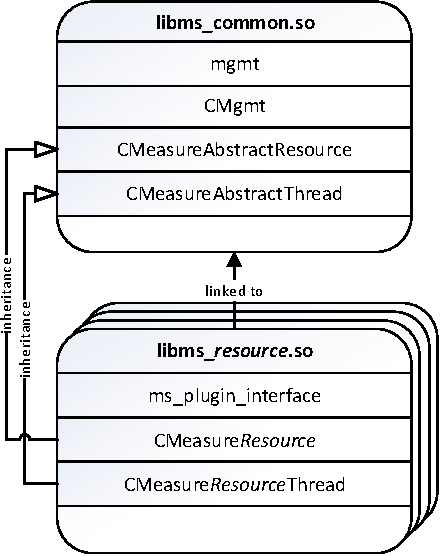
\includegraphics[width=0.4\textwidth]{libmeasure_princip} 
\caption{Design concept of the libmeasure software architecture. Each resource-specific module has to inherit from two abstract classes. Since the resource modules are dynamically loadable modules which can be loaded at runtime, they have an C interface to access the module (\texttt{ms\_plugin\_interface}).}
\label{fig:libmeasure_principle}
\end{center}
\end{figure}

\begin{description}
	
	\item[\texttt{libms\_common.so}] contains resource-independent classes with some abstract methods which have to be implemented in inherited classes encapsulated in the resource-specific modules. Moreover, there are other classes which are common to all resource-specific modules. These classes are needed for the module management, library initialization, and so on.

\pagebreak
\vspace*{-1.0cm}

	\begin{itemize}
		\item \texttt{CMeasureAbstractResource}: Abstract class for the measurement functionality of a resource. This class is used as skeleton for the concrete measurement class which is responsible to obtain the measurement values. Therefore this class provides a virtual \texttt{measure()} method which must be implemented by all resource-specific modules. Our measuring library calls the non-virtual \texttt{measure()} method of the inherited resource-specific class, if the time slot given by the resource's sampling rate is expired.
		
		\item \texttt{CMeasureAbstractThread}: Abstract class for the thread which periodically executes the \texttt{measure()} function for one resource in its inherited resource-specific classes. All thread management functions such as \texttt{start()}, \texttt{stop()}, or \texttt{join()} are implemented in this abstract class and must not be overwritten in the functions of the inherited classes.
		On the other side, the \texttt{run()} method of the thread is abstract and needs to be implemented in the concrete implementation in \texttt{libms\_resource.so}. This class also enables controlling of the actual measurement threads, i.e., it initializes and stops the threads which trigger the resource-dependent \texttt{measure()} methods.
		
		\item \texttt{CMgmt}: This class is responsible for the management of all measurements. All POSIX-Threads executing the measuring procedures in the inherited implementations of \texttt{CMeasureAbstractThread} are instantiated in this class (in fact, the raw POSIX-Thread handling is performed in the \texttt{CMeasureAbstractThread} class and its children). In its constructor every module is dynamically loaded with \texttt{dlopen()}. This is still implemented statically. In the future, we are going to reimplement the module loader in a more dynamic way, so that modules are only loaded, if they are listed in a configuration file located in the user's home directory.
		
		\item \texttt{mgmt}: This class implements the libmeasure management functions such as \texttt{ms\_init()}, \texttt{ms\_start\_measurement()} or \texttt{ms\_join\_measurement()} which can be called from C. We describe this functions in Section \ref{sec:libmeasureUsage}. These functions are accessible by including the corresponding interface header file \texttt{measurement.h}.
	\end{itemize}
	
	\item[\texttt{libms\_resource.so}] encapsulates a resource-specific module with the concrete implementation of the abstract classes which are compiled to the shared object \texttt{libms\_common.so}. As already mentioned, the word \textit{resource} is used as a template and must be replaced by a concrete resource. We  illustrate the structure of the resource-specific modules without considering the real class names but using the template word \textit{resource}. Feel free to take a look to the source code for better understanding of the modules, respectively plugins.\\
	Every resource with sensors that should be sampled by the libmeasure, must have a separate module with implementations of the abstract classes mentioned in the prior passage. Since the modules are loaded like plugins, there must be an implementation of the plugin interface, too.
	\begin{itemize}
		\item \texttt{CMeasureResource}: Implementation of the abstract class\\\texttt{CMeasureAbstractResource} and therefore also the \texttt{measure()} method. The resource-specific measuring functionality is implemented and all retrieved values are stored in the \texttt{MEASUREMENT} struct. No further calculations such as the integration of the retrieved power data to get the consumed energy since the last sample are done here. Such computations are done in the \texttt{run()} method of \texttt{CMeasureResourceThread}, i.e., the \texttt{run()} method calls the \texttt{measure()} method periodically, calculates additional data such as the consumed energy from raw power data stored in the \texttt{MEASUREMENT} struct, and finally stores these results in other elements of the \texttt{MEASUREMENT} struct. Furthermore, all resource-specific initialization should be done in the constructor of the \texttt{CMeasureResource} class (e.g. calling the external library NVML which is used for sampling sensors of Nvidia GPUs). Consequently, the destructor is used to close the libraries and/or free the memory allocated for using the libraries. \added[id=al]{The class provides two templates for flexible and easily customizable measurements. The first template parameter \texttt{TSkipMs} is used to decrease the number of sensor readings for measurement procedures which cause high CPU utilization. The second template parameter \texttt{TVariant} is a switch to select the \texttt{LIGHT} or \texttt{FULL} library variant.} \added[id=al]{Können wir da ein T an den Beginn der Parameter setzen, also TSkipMS?}
		
		\item \texttt{CMeasureResourceThread}: Concrete implementation of\\ 
		\texttt{CMeasureAbstractThread} and therefore the resource-specific \texttt{run()} method. This class uses the \texttt{CMeasureResource} class to retrieve measurement values periodically. The \texttt{run()} method basically consists of a loop frequently calling the \texttt{measure()} method of the \texttt{CMeasureResource} class. Afterwards all necessary calculations such as accumulation of energy values are done with the obtained values which are located in the \texttt{MEASUREMENT} struct. The \texttt{measure()} method only stores values which can be directly read from the sensors placed on-die or on-board of the resources. The further processing of the raw data is then performed in the loop of the \texttt{run()} method located in \texttt{CMeasureResourceThread} or after the loop before thread termination. For example, the recently measured power dissipation and time slice since the last sampling (approximately the sampling rate) are used to calculate the energy consumed during this period. Finally, this intermediate result is used to accumulate/sum up the total energy consumption during the whole measurement respectively between calling \texttt{ms\_start\_measurement(ms, m)} and \\\texttt{ms\_stop\_measurement(ms, m)} (Section \ref{sec:libmeasureUsage}). The calculated values are stored in the \texttt{MEASUREMENT} struct again. \added[id=al]{This templated class has the same template parameter \texttt{TVariant} as imlemented in the \texttt{CMeasureResource} class. The parameter is used to omit calculations unnecessary for the libmeasure \texttt{LIGHT} variant. For example, the maximum temperature is not computed since the temperature queries are disabled in the \texttt{LIGHT} variant.}
		
		\item \texttt{ms\_plugin\_interface}: This is the C interface of the module respectively plugin which is called from the \texttt{CMgmt} class in order to instantiate the \texttt{CMeasureResource} and \texttt{CMeasureResourceThread} objects. Since the interface is written in C but the library encapsulates C++ classes, the returned void pointers are usually related to objects.
	\end{itemize}
\end{description}

Figure \ref{fig:libmeasureSequence} illustrates in which way the classes interact in order to perform the measurements. Moreover, there is a rough overview of the topmost functions users have to call in order to use libmeasure (functions with \texttt{ms\_} prefix). For simplification only one resource is shown. Therefore, the keyword \textit{Resource} is used again.\\

\begin{figure}
\begin{center}
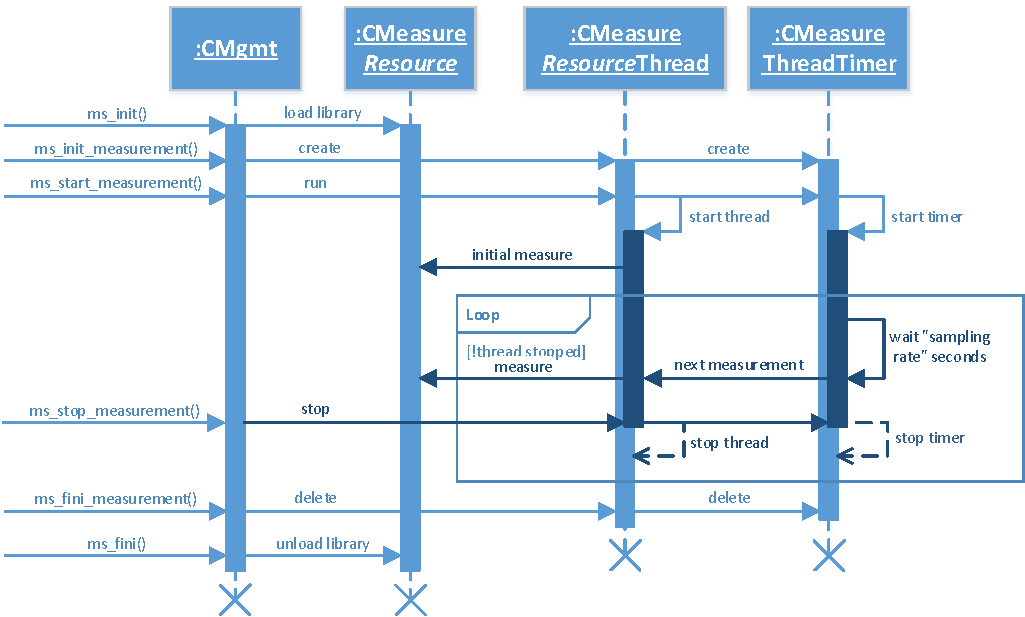
\includegraphics[width=0.8\textheight, angle=-90]{ampehreSequence} 
\caption{Libmeasure sequence diagram showing the interactions between different objects of the library. Please note that the figure illustrates a simplified representation.}
\label{fig:libmeasureSequence}
\end{center}
\end{figure}

On the one side, all resource-specific libraries have to be linked against the \texttt{libms\_common.so}. On the other side, \texttt{libms\_common.so} does not need to be linked against the resource-specific implementations. This is not necessary, because the \texttt{CMgmt} class \textit{dynamically loads the modules at runtime like plugins}, calls the interface, obtains the module-internal objects as void pointers, and stores the objects in their abstract types. Since we dynamically load the resource-specific shared objects at runtime, we have to compile the modules as dynamically loadable modules. Take a look to the \texttt{CMakeLists.txt} files to see how to compile appropriately.\\

Figure \ref{fig:libmeasure_overview} shows the libmeasure with all currently available modules. There you can also see the replacement of \textit{resource} by real class names. All modules have the same structure and implementations of the abstract classes from the \texttt{libms\_common.so}. Caused by some ``historic'' reasons, our naming scheme is inconsistent. For instance, instead of naming the \texttt{CMeasureResource} and \texttt{CMeasureResourceThread} classes in \texttt{libms\_gpu\_nvidia\_tesla\_kepler.so} \\\texttt{CMeasureGPU} and \texttt{CMeasureGPUThread}, we used the name of the library (NVML) that we utilize to retrieve the measurement values.\\

As we already mentioned in Section \ref{sec:BuildInstallInstructions}, it is possible to build and install the project with a subset of supported resources. In this case the module \texttt{libms\_stub.so} is loaded instead of the disabled resource-specific modules. The stub module has no functionality but defines all necessary classes and functions. This allows loading the stub module in the \texttt{CMgmt} class like all other modules. If the functions are called, no measurement thread is created and the values stored to the \texttt{MEASUREMENT} struct are always zero.

\begin{figure}
\begin{center}
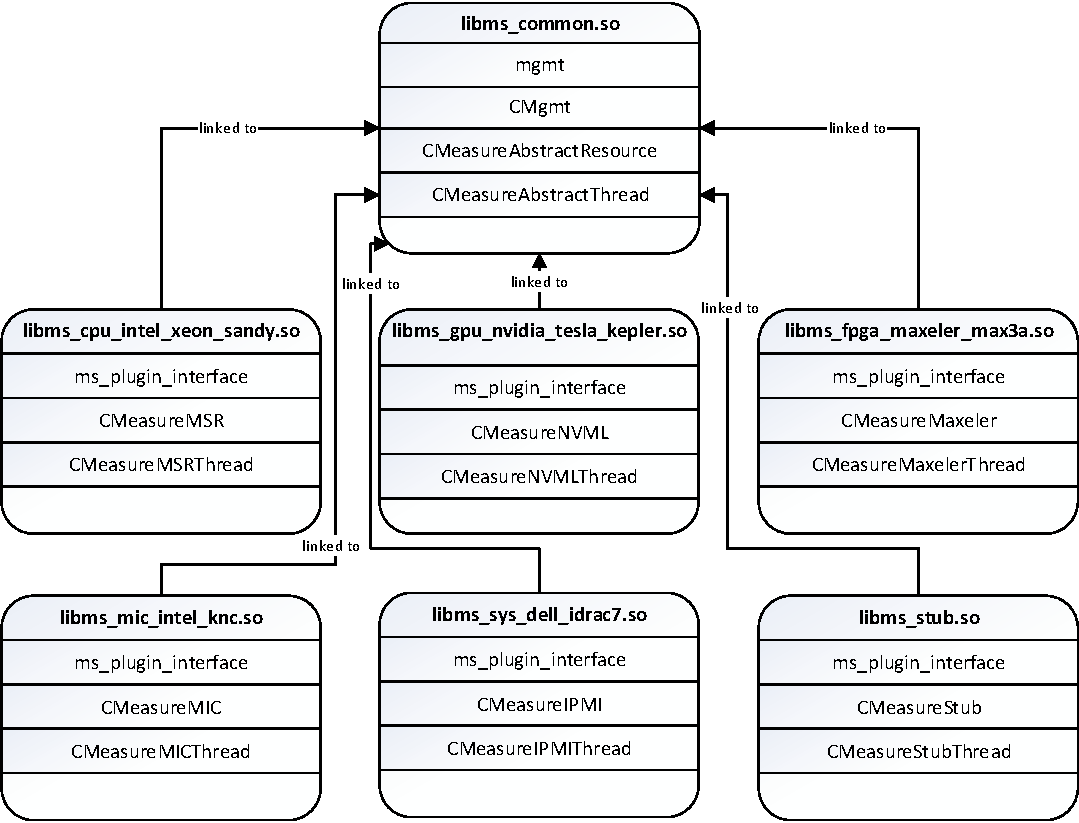
\includegraphics[width=\textwidth]{libmeasure} 
\caption{Overview of libmeasure with all available modules.}
\label{fig:libmeasure_overview}
\end{center}
\end{figure}

\pagebreak

\subsection{Modular Expendability}
The existing modules fit perfectly to our heterogeneous node but it is very unlikely that someone uses a system with the same hardware resources. Therefore the modular software architecture can be extended by additional modules for new or different resources. In the following section, we explain how new modules must be implemented and what programmers have to modify in the \texttt{libms\_common.so} to add a new module. Since you must modify the code of \texttt{libms\_common.so}, this shared object is not really resource-independent at the moment. In one of our next future releases, we will address this issue, so that programmers must only provide a plugin without any changes to other code segments of Ampehre. \added[id=al]{Since version 0.6.0 we use C++ templates in all of our modules to provide an easily adjustable measuring framework as introduced in Section \ref{sec:SoftwareArchitecture}. In the following sections we describe how to add a new resource to libmeasure. This includes how to use the introduced templates in your individual extension as well.} The following list shows all files and classes of the libmeasure which have to be edited or added.

\begin{itemize}
	\item \textbf{resource-specific module:}
	\begin{itemize}
		\item \texttt{ms\_plugin\_interface}
		\item \texttt{CMeasureResource}
		\item \texttt{CMeasureResourceThread}
		\item \texttt{CMakeLists.txt}
	\end{itemize}
	\item \texttt{measurement.h}
	\item \textbf{libms\_common.so:}
	\begin{itemize}
		\item \texttt{interface.cpp}
		\item \texttt{CMgmt}
		\item \texttt{mgmt.cpp} 
	\end{itemize}
\end{itemize}
In the following sections, we discuss each modification in detail. Please feel free to use the existing modules as examples to create new modules.

\subsubsection{Resource-specific module}
For a complete module, we recommend to implement six source files and a \texttt{CMakeLists.txt}. Please, add a directory for each new module. In order to build your module together with our modules you should add the name of your module's directory to the \texttt{CMakeLists.txt} in the libmeasure folder by using the \texttt{add\_subdirectory()} cmake instruction.
\begin{description}
	\item[ms\_plugin\_interface] is the implementation of the C interface to the module/plugin. The interface is identical for every module and the corresponding unique header file is \texttt{/include/ms\_plugin\_interface.h}. The functions necessary to implement this interface are shown in Listing \ref{lst:ResourceInterface}.
	
	\begin{lstlisting}[caption={Interface that each plugin must implement.\added[id=ck]{Listing aktualisiert.}}, label=lst:ResourceInterface]
void* init_resource(void* pLogger, void* pParams);
void  fini_resource(void* pMeasureRes);

void* init_resource_thread(void* pLogger, void* pStartSem,
						   MEASUREMENT* pMeasurement,
						   void* pMeasureRes);
void  fini_resource_thread(void* pMeasureResThread);

void  trigger_resource_custom(void* pMeasureRes,
							  void* pParams);
	\end{lstlisting}
	The init functions create an object of the \texttt{CMeasureResource} or \\ \texttt{CMeasureResourceThread} class and return it as a void pointer. The fini functions get these objects as void pointers and delete the objects.
	The additional parameter \texttt{void* pParams} of the \texttt{init\_resource()} function can be used to pass an arbitrary number of parameters to the \\\texttt{CMeasureResource} object during the initilization. \added[id=ck]{The first and second parameters stored in \texttt{pParams} are always the enums which select the values of the templates \texttt{int SkipMs} and \texttt{int Variant} of the \texttt{CMeasureResource} class. The template \texttt{int Variant} of the \texttt{CMeasureResourceThread} needed in the \texttt{init\_resource\_thread()} function is selected according to the variant of the \texttt{CMeasureResource} object.} \added[id=al]{Welche enums? Das kann man doch sicher einfacher erklären. Wenn die werte immer gegeben sind, sollten wir die nicht auslagern in eigene Variablen, statt in pParams zu packen? Hier sollten auch Referenzen auf Chapter 3 eingefügt werden, da dort alles wesentliche schon geklärt wird. Außerdem werden hier einfach zwei Templateparameter verwendet ohne eingeführt zu sein. Abstrakter formulieren.} While the init and fini functions are mandatory for a new module, the function \texttt{trigger\_resource\_custom()} is optional and can be used to call any custom function for a specific resource. For example, we use this function to process a ``force idle function'' of the FPGA, which is used to reconfigure the FPGA with an empty bitstream. If you do not need the additional custom function add it anyway but keep the function body empty.
	
	\item[CMeasureResource] extends the class \texttt{CMeasureAbstractResource} and therefore has to implement the methods shown in Listing \ref{lst:CMeasureResource}. \added[id=ck]{This class has a template \texttt{int SkipMs} to define which measurements in the \texttt{measure()} method can be performed with a lower frequency and a second template \texttt{int Variant} to select which measuring values should be obtained.} \added[id=al]{This class provides to template parameters. First is used for... (TSkipMs) second is good for... (TVariant).}
	\begin{lstlisting}[caption={Methods of the \texttt{CMeasureResource} class that programmers have to implement in order to support a new resource. \added[id=ck]{Listing aktualisiert.}}, label=lst:CMeasureResource]
private:
	void init(void);
	void destroy(void);
	
public:
	void measure(MEASUREMENT *pMeasurement, 
				int32_t& rThreadNum);
	int  getVariant();
	\end{lstlisting}
	
	The method \texttt{init()} is used to initialize the libraries needed to obtain the measurement values from the resources. For example in our GPU module we initialize the NVML, open the device, store the pointer to the device for later queries and set the frequencies to the desired values. This allows it to query the measurement values after the initialization from the resource without any unnecessary overhead. Furthermore the \texttt{init()} method can be used to display the capabilities of the resource on which the measurements are performed. An example is our CPU module where all available CPU frequencies are displayed.\\
	After the last measurement, all used libraries need to be closed and the allocated memory must be freed. Therefore we provide a \texttt{destroy()} method which is similar to \texttt{init()}. For example, in our GPU module we set the clock frequencies back to the default values and close the NVML environment.\\
	The method \texttt{measure()} is called to obtain the current measurement values from the resource. Every value which is measured here needs to be stored in the \texttt{MEASUREMENT} struct which is passed as parameter to the method. The extension of the \texttt{MEASUREMENT} struct to store additional values is explained later. The second parameter of the \texttt{measure} method is the thread id of the thread which executes this method. The thread ids are used for a first debugging without professional debuggers such as gdb. \added[id=ck]{In the \texttt{measure} method the template \texttt{int Variant} is used in an conditional block to select which measurements should not be performed in certain variants of the library. For example some measurements are only performed if \texttt{Variant} has the value \texttt{FULL}. The template \texttt{SkipMs} is used in combination with the member variable \texttt{mMeasureCounter} to  peform some measurments not at every call to the \texttt{measure()} method. Listing \ref{lst:CMeasureResourceMeasure} shows an example how the templates are used.} \added[id=al]{Verweise auf Tabelle Chapter 3. Bitte prüfen: measurment vs. measurEment. Ich würde die beiden Template parameter konkret auf Listing 11 beziehen und ein Beispiel verwenden. Das hier hört sich sehr generisch/"Füllsatz"-mäßig an. Und für was verwenden wir mMeasureCounter? Wird nicht verständlich.}
	
	\begin{lstlisting}[caption={\added[id=ck]{Abstract minimal example for the \texttt{measure()} method of the \texttt{CMeasureResource} class to clarify the use of the templates.}\added[id=al]{Im generischen Text oben, wird das eben nicht clarified.}}, label=lst:CMeasureResourceMeasure]
template <int SkipMs, int Variant>
void CMeasureResource<SkipMs, Variant>::measure(MEASUREMENT* pMeasurement, int32_t& rThreadNum) {
	//This measurements are always performed.
	ResourceGetPower(pMeasurement, rThreadNum);
	ResourceGetUtil(pMeasurement, rThreadNum);

	if(Variant == FULL) {
		// This is only executed in the FULL variant.
		ResourceGetFrequency(pMeasurement, rThreadNum);
		if(!(mMeasureCounter++ % SkipMs)) {
			//This is executed every SkipMs'th call. 
			ResourceGetMemory(pMeasurement, rThreadNum);
			ResourceGetTemperature(pMeasurement, rThreadNum);
		}
	}
}
	\end{lstlisting}
	\added[id=ck]{The method \texttt{getVariant()} returns the value of the template \texttt{Variant}. This method is needed to instantiate the \texttt{CMeasureResourceThread} with the same value for the template.}\added[id=al]{Kann man sich sparen bei get/set Funktionen.}
	 
	\item[CMeasureResourceThread] extends the class \texttt{CMeasureAbstractResource} and thus has to implement the \texttt{run()} method as shown in Listing \ref{lst:CMeasureResourceThread}. \added[id=al]{Please note, that this class has the same template \texttt{TVariant} as described for the \texttt{CMeasureResource} class. It is used to omit some calculation which are not needed for the libmeasure \texttt{LIGHT} variant.}
	\begin{lstlisting}[caption={Methods of the \texttt{CMeasureResourceThread} class that programmers have to implement in order to support a new resource.}, label=lst:CMeasureResourceThread]
private:
	void run(void);
	\end{lstlisting}
	The method \texttt{run()} is the centerpiece of the \texttt{CMeasureResourceThread} class. At the beginning, all values in the measurement struct related to the resource need to be set to zero, especially those which are used as accumulators. Moreover the method needs to follow the structure shown in Listing \ref{lst:RunMethodScheme}.
	
\pagebreak
\vspace*{-2.6cm}

\begin{lstlisting}[caption={Scheme of the \texttt{run()} method that each \texttt{CMeasureResourceThread} must have. \added[id=ck]{Listing aktualisiert}}, label=lst:RunMethodScheme]
template <int Variant>
void CMeasureResourceThread::run(void) {
	mThreadStateRun		= true;
	mThreadStateStop	= false;
	uint64_t skip_ms_cnt = 0;
	mThreadNum = CThread::sNumOfThreads++;
	
	mMutexTimer.lock();
	
	// Set all values in the measurement struct to zero.
	...
	
	mpMutexStart->unlock();
	mrStartSem.wait();
	
	// First initial measurement. 
	mrMeasureResource.measure(mpMeasurement, mThreadNum);
	
	while (!mThreadStateStop) {
		/*
		 * This mutex is used to synchronize the while
		 * loop with a timer. The timer unlock the mutex
		 * every sampling rate seconds.
		 */
		mMutexTimer.lock();
		
		/*
		 * Here the measure method of the class
		 * CMeasureResource is called dependent on
		 * the skip_ms_rate.
		 */
		if(!(skip_ms_cnt++ % mpMeasurement->skip_ms_rate)){
			mrMeasureResource.measure(mpMeasurement,
									  mThreadNum);
		}
		
		/*
		 * Calculates the difference between the current time
		 * and the last stored time and returns the result
		 * in time_diff and time_diff_double. Note, that the
		 * calculated time always differs from the sample
		 * rate. We decided to have this second time
		 * information to compute energy in a more precise
		 * way.
		 */
		calcTimeDiff(&(mpMeasurement->
				       	internal.resource_time_cur),
					 &(mpMeasurement->
					 	internal.resource_time_temp),
					 &(mpMeasurement->
						 internal.resource_time_diff),
					 &(mpMeasurement->
						 internal.resource_time_diff_double));
			
		/* 
		 * Calculate results here and store everything
		 * in the measurement struct.
		 */
		...
		
		if(Variant == FULL) {
			/*
			 * Remember to differentiate between the variants.
			 * Here calculations which are only needed in the
			 * full variant are done.
			 */
		}
		
	}
	
	/* 
	 * Calculate some additional results such as average
	 * power dissipation on the base of consumed energy
	 * and store the results in the measurement struct.
	 */
	...
	
	// Thread termination
	exit();
}	
\end{lstlisting}
	The mutex \texttt{mMutexTimer} gets locked in every loop run. We have implemented a timer thread which is part of the \texttt{libms\_common.so} to unlock this mutex dependent on the sampling rates. The timer thread is a member of the \texttt{CMeasureAbstractResource} class but should be configured as shown in Listing \ref{lst:CMeasureResourceThreadConstructor}. Please replace the string of \texttt{setThreadName()} with a custom resource-dependent string. In addition, set the timer with a resource-dependent sampling rate stored in a variable in the \texttt{MEASUREMENT} struct. Finally, you must share the mutex of the \texttt{CMeasureResourceThread} class with the timer. This is mandatory as this mutex is used for synchronization as explained above.

\begin{lstlisting}[caption={\texttt{CMeasureResourceThread} constructor template.},label=lst:CMeasureResourceThreadConstructor]
mTimer.setThreadName("Resource timer");
mTimer.setTimer(&(pMeasurement->resource_time_wait));
mTimer.shareMutex(&mMutexTimer);
\end{lstlisting}
	
	\item[CMakeLists.txt] compiles all source files to one dynamically loadable library and links the module against the provided \texttt{libms\_common.so} library. Finally, as already mentioned above, you must add the directory containing the new module and the if statement for the new module to the \texttt{CMakeLists.txt} located in the \texttt{/libmeasure} directory. Code for the new module in the \texttt{CMakeLists.txt} should look like the already existing. We also need to add a new option for the module to the \texttt{CMakeLists.txt} of the project root directory as shown in Listing \ref{lst:CMakeListsResourceSupport}.
\end{description}

\subsubsection{measurement.h}
\label{sec:measurement_h}
For a new resource a define preprocessor directive has to be added to the header \texttt{measurement.h}. We assign a single integer to each resource. The i-th resource gets the value $2^{i}$, so that each bit of the integer indicates one specific resource. Moreover the new resource needs a define directive which indicates whether the library or the stub should be loaded. The define preprocessor directive in the ifdef-statement is triggered dependent on the options set in the \texttt{CMakeLists.txt} file of the project's root directory (Listing \ref{lst:CMakeListsResourceSupport}). This preprocessor directive \texttt{Resource\_LIB} will only be true if the library is compiled with support for the corresponding resource. The edited header including the new resource could look like Listing \ref{lst:measurement.h_defines}.
\begin{lstlisting}[caption={Extended \texttt{measurement.h} header file with new define directives to support a new resource.},label=lst:measurement.h_defines]
#define CPU		 0x01
#define ...
#define RESOURCE 0x20
#define ALL		(CPU | GPU | GPU | FPGA | SYSTEM | MIC | RESOURCE)
		
#ifdef Resource_LIB
	#define Resource_LIB_NAME "libms_resource.so"
#else
	#define Resource_LIB_NAME "libms_stub.so"
#endif
\end{lstlisting}
The \texttt{MEASUREMENT} struct is also defined in \texttt{measurement.h}. For every value which should be measured, a new variable needs to be added here. Furthermore the methods to obtain the measured values after stopping the measuring procedure are declared here. For this, you have to add a function for each value of interest stored in the struct. Supplementary variables to store the sampling rate and the skip rate, set by the call to \texttt{ms\_set\_timer()} during the initialization need to be added to the \texttt{MEASUREMENT} struct as shown in Listing \ref{lst:measurement.h_struct}.
\begin{lstlisting}[caption={Mandatory extensions for the \texttt{MEAUSREMENT} struct defined in \texttt{measurement.h}.},label=lst:measurement.h_struct]
struct timespec resource_time_wait;
uint32_t resource_skip_ms_rate;
\end{lstlisting}
Temprorarily variables which are needed for the calculation of other measurement results can be added to the C struct \texttt{MEASUREMENT\_INTERNAL}. Furthermore, you need to add new variables to the internal struct to store time stamps for the new resource. These timespec structs are used to hold precise time information and can be used to calculate energy out of measured power values. The additions to the internal struct should look like the code shown in Listing \ref{lst:measurement.h_internal_struct}.
\begin{lstlisting}[caption={Extensions for the \texttt{MEAUSREMENT\_INTERNAL} struct defined in \texttt{measurement.h}.}, label=lst:measurement.h_internal_struct]
struct timespec resource_time_cur;
struct timespec resource_time_temp;
struct timespec resource_time_diff;
double resource_time_diff_double;
\end{lstlisting}

\subsubsection{libms\_common.so}
You have to modify some files which are compiled and bundled to the \texttt{libms\_common.so} library. The necessary modifications are described in the following paragraphs. \texttt{libms\_common.so} should be resource-independent. For this, we will remove all resource-specific code from the library in one of the next releases of Ampehre.

\begin{description}
\item[interface.cpp] implements the interface to obtain all measured values as well as data that are calculated in the \texttt{CMeasureResourceThread}s. For each of these values, a function declaration must be added to \texttt{measurement.h} and the corresponding function definition must be added to the \texttt{interface.cpp} file. These functions are used to return the measured values stored in the \texttt{MEASUREMENT} struct. The \texttt{MEASUREMENT} struct should be the first parameter of the functions. The following listing shows an example for a function returning the total/accumulated energy consumed during a measuring.
\begin{lstlisting}[caption={Example for a function to return values stored in a \texttt{MEASUREMENT} struct.}, label=lst:GPUEnergyExample]
double gpu_energy_total(MEASUREMENT *measurement) {
	return measurement->nvml_energy_acc;
}
\end{lstlisting}

\item[CMgmt] is the link between the C user interface and the resource-specific threads and thus provides functions to control the measurement threads (take a look at Figure \ref{fig:libmeasureSequence}). The class \texttt{CResourceLibraryHandler} is used to dynamically load a module with \texttt{dlopen()}, initializes the resource-specific object \texttt{CMeasureResource} and stores it as a pointer. The \\\texttt{CResourceLibraryHandler} calls the plugin interface and provides functionality to execute any of the plugin interface functions via \texttt{dlysm()}. Each resource-specific module such as \texttt{CMeasureResource} is instantiated in \texttt{CMgmt} and is stored for later access. The \texttt{CResourceLibraryHandler} gets the module name passed as parameter in the constructor. It automatically loads the module and instantiates a \texttt{CMeasureResource} object. \added[id=ck]{The last parameter of the \texttt{CResourceLibraryHandler} constructor is used to pass all parameters as \texttt{void*} to the \texttt{CMeasureResource} class of the new module. The first parameter is always the value for the template \texttt{Variant} and the second parameter is the value for the template \texttt{SkipMs} of the \texttt{CMeasureResource}. After this any number of additional parameters can be passed to the \texttt{CMeasureResource}.} \added[id=al]{Siehe oben: Variant und Skip separieren von Params?} For example, we use this parameter to set the GPU clock frequencies. The \texttt{CResourceLibraryHandler} object for the new modules is inserted to the data container \texttt{mResources} which is a member of the \texttt{CMgmt} class.\\
\added[id=ck]{Listing \ref{lst:CMgmtExtension} shows what needs to be added to the constructor in order to add a new module. In this example we pass the template values and additionaly the GPU frequency settings to the \texttt{CMeasureResource}.} \added[id=al]{Siehe oben.}
\begin{lstlisting}[caption={Extension to the \texttt{CMgmt} constructor. \added[id=ck]{Listing aktualisiert}}, label=lst:CMgmtExtension]
uint64_t params_gpu[] = {mLibVariant, skip_ms, gpuFrequency};
mResourceVector.insert(mResourceVector.begin() + 
				(int)log2(RESOURCE),
				new NLibMeasure::CResourceLibraryHandler(
				mLogger, RESOURCE_LIB_NAME,
				(void*)	params_gpu));
\end{lstlisting}

\item[mgmt.cpp] is the implementation of the C interface to the library management functionality. Functions such as \texttt{ms\_init\_measurement()} and\\ \texttt{ms\_start\_measurement()} (Section \ref{sec:libmeasureUsage}) which are declared in \texttt{measurement.h} are defined in the \texttt{mgmt.cpp} file. Three functions have to be modified in order to integrate a new resource to \texttt{libms\_common.so} respectively libmeasure. The first function is \texttt{ms\_set\_timer} where the sampling rates for each resource are set. This defines how often the \texttt{measure()} function of the class \texttt{CMeasureResource} is called in the \texttt{run()} method of \\\texttt{CMeasureResourceThread}. Therefore the switch statement has to be extended by a new case as indicated in the next listing. The identifier of the case statement is defined in \texttt{measurement.h} (Listing \ref{lst:measurement.h_defines} of Section \ref{sec:measurement_h}).
\begin{lstlisting}[caption={Code to store resource-specific sampling rates in the \texttt{ms\_set\_timer()} function. \added[id=ck]{Listing aktualisiert}}, label=lst:mgmt]
case RESOURCE:
	measurement->resource_time_wait.tv_sec	= sec;
	measurement->resource_time_wait.tv_nsec	= nsec;
	measurement->resource_skip_ms_rate  	= skip_ms_rate;
	break;
\end{lstlisting}
The second function which has to be modified is \texttt{ms\_init\_measurement()}. Here you must add an if statement which is needed for appropriate plugin instantiation. An example is listed in Listing \ref{lst:mgmtMsInitMeasurement}.
\begin{lstlisting}[caption={Extension of the \texttt{ms\_init\_measurement()} function.}, label=lst:mgmtMsInitMeasurement]
if (flags & RESOURCE) {
	ms->initMeasureThread(RESOURCE, measurement);
}
\end{lstlisting}

The third function which has to be modified is \texttt{ms\_alloc\_measurement()}. You should set the \texttt{struct timespec} which holds the sampling rate to maximum \added[id=ck]{and the \texttt{skip\_ms\_rate} to the default value one.} \added[id=al]{Vllt. sollten wir einen besseren Bezeichner hierfür verwenden. Es gibt zwei "Skips": Skipping some measurements in measure function and skipping some measurements at all (LIGHT).}
\begin{lstlisting}[caption={Extension of the \texttt{ms\_alloc\_measurement()} function.}, label=lst:AlloctoMaxInteger]
measurement->resource_time_wait.tv_sec		= UINT64_MAX;
measurement->resource_time_wait.tv_nsec		= UINT64_MAX;
measurement->resource_skip_ms_rate			= 1;
\end{lstlisting}
\end{description}

